% !TeX root = ../../main.tex
% !TEX spellcheck = en_GB

\section{Design}
\label{ch:Design}
\fxnote{Detailed diagram. Discussion of issues and thoughts on how they have been solved/will influence the system.}

To fulfil the requirements specified, the system is split into three parts: Preprocessing, Signal processing and Post processing, as seen in \cref{fig:overalldesign}.

\paragraph{Preprocessing} handles the analog to digital conversion and preprocessing allowing compliance with Non-functional requirement R1 and R2 for the Signal processing block.
This means Preprocessing takes the input, processes it and outputs a sample frequency and buffer size whose ratio allows for frequency bins smaller than \SI{2.5}{\hertz}.

\paragraph{Signal processing} finds the frequency/tone to move and moves it to the corresponding C-major tone.

\paragraph{Post processing} ensures the sound quality is maintained after Preprocessing and Signal processing.

\begin{figure}
	\centering
	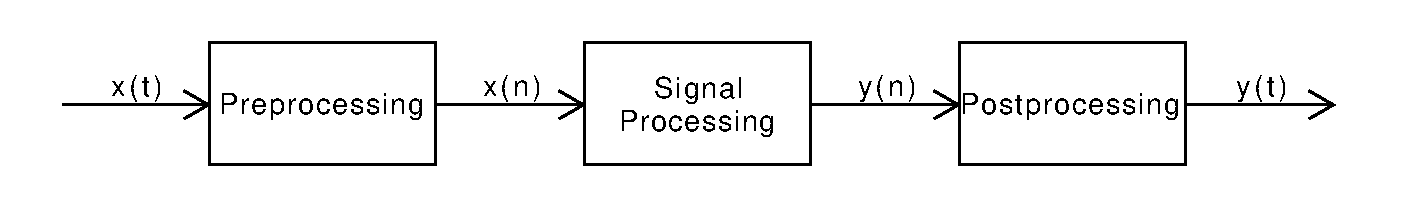
\includegraphics[width=1\linewidth]{gfx/Design/OverallDesign.pdf}
	\caption{Overall design of \systemName.}
	\label{fig:overalldesign}
\end{figure}


\FloatBarrier